\documentclass[a4paper,12pt]{article}
\usepackage[utf8]{inputenc}
\usepackage{graphicx}
\usepackage{hyperref}
\setlength\emergencystretch{\hsize}\hbadness=10000

\title{Comparação de Modelos TTS: XTTS vs. YourTTS}
\author{
  Aluno: Thomaz Diniz Pinto de Morais\\
  \texttt{thomaz.morais@ccc.ufcg.edu.br}
  \and
  Orientador: Herman Martins Gomes\\
  \texttt{hmg@dsc.ufcg.edu.br}
}
\date{}

\begin{document}

\maketitle

\section{Introdução}
	A síntese de voz (TTS) é uma tecnologia essencial para diversas aplicações, como assistentes virtuais, leitura automática de textos, e acessibilidade. Este estudo visa replicar parcialmente o artigo "Conversão Texto-Fala para o Português Brasileiro Utilizando Tacotron 2 com Vocoder Griffin-Lim" \cite{rosa2021ttsptbr}. Nele os autores se utilizam de um conjunto de dados chamado Common Voice para treinar o modelo Tacotron e gerar audio em português brasileiro. 
 

\section{Metodologia}

	Neste artigo utilizaremos uma implementação \textit{TTS} disponibilizada pela \textit{coqui-ai}\footnote{Repositório no GitHub: \url{https://github.com/coqui-ai/TTS}} para comparar modelos de \textit{TTS} multilinguais na lingua portuguesa do Brasil. Os modelos selecionados são o \textit{XTTS} e o \textit{YourTTS}, ambos modelos já capazes de sintetizar vozes em português brasileiro.
	Rosa et. al. \cite{rosa2021ttsptbr} avalia seu modelo através da contagem da quantidade de erros de pronúncia e de palavras ignoradas. Neste artigo avaliaremos utilizando a mesma contagem de erros e com as mesmas sentenças sintetizadas pelo modelo do artigo original. Para isto, sintetizamos as 200 sentenças que foram disponibilizadas pelo artigo de Rosa et. al. para os dois modelos que selecionamos (\textit{XTTS} e \textit{YourTTS}) e, posteriormente, fizemos a contagem da quantidade de erros de pronúncia e palavras ignoradas pelo sintetizador.
	
\section{Reprodução}

	Para sintetização de voz utilizamos a implementação disponível no repositório do github da \textit{coqui-ai}. Desenvolvemos também um passo-a-passo de como executar os códigos para sintetização das sentenças. O resultado disso está disponível em um repositório do github\footnote{Repositório no GitHub: \url{https://github.com/ThomazDiniz/tts}}, bem como os áudios sintetizados, e uma página com resultados e demonstração dos áudios sintetizados.  Ao finalizar a sintetização das sentenças, fizemos a avaliação das sentenças uma a uma manualmente. Escutando o resultado e verificando se houveram erros de português e palavras ignoradas pelo sintetizador de voz.

	Os dois modelos , \textit{XTTS} e \textit{YourTTS}, foram avaliados com as mesmas 200 sentenças do artigo de Rosa et al. Fizemos a contagem de erros de pronúncia de forma manual e registramos os seguintes resultados:

\begin{table}[h!]
\centering
\begin{tabular}{|c|c|c|}
\hline
Tipo de Erro & \textit{XTTS} & \textit{YourTTS} \\ \hline
Palavras puladas & 0 & 0 \\ \hline
Erros de pronúncia & 10 & 50 \\ \hline
\end{tabular}
\caption{Comparação dos resultados entre \textit{XTTS} e \textit{YourTTS}}
\label{tab:my_table}
\end{table}


\begin{figure}[h!]
\centering
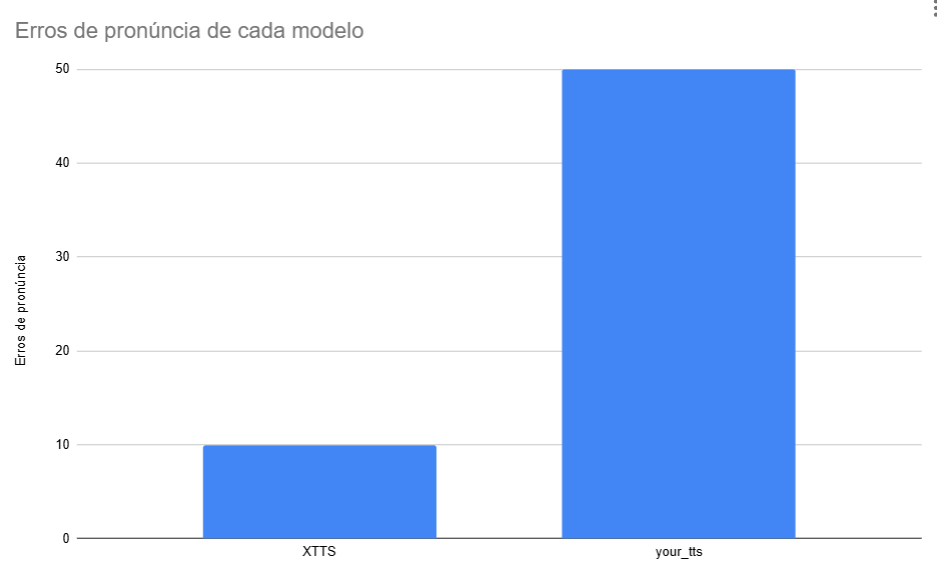
\includegraphics[width=0.8\textwidth]{imgs/histograma_erros.png}
\caption{Comparação dos erros de pronúncia entre os modelos XTTS e YourTTS.}
\label{fig:comparison}
\end{figure}


\section{Conclusões}
Os resultados obtidos, bem como alguns dos áudios sintetizados podem ser observados em uma \textit{github page} dedicada aos resultados desta reprodução\footnote{Página no GitHub Pages: \url{https://thomazdiniz.github.io/tts/}}. Os resultados nos mostram que o modelo XTTS tem uma precisão de pronúncia significativamente melhor em comparação ao YourTTS. A baixa taxa de erros de pronúncia no XTTS indica uma performance superior, tornando-o uma opção mais viável que o YourTTS.

	\bibliographystyle{ACM-Reference-Format}
	\bibliography{ref}
	
\end{document}